
\documentclass[12pt,reqno]{amsart}

\usepackage{amsmath}
\usepackage{amsfonts}
\usepackage{amssymb}

\usepackage{graphicx}
%\usepackage{epstopdf}
\usepackage[colorlinks=true]{hyperref}
\usepackage[left=1in,right=1in,top=0.9in,bottom=0.9in]{geometry}
\usepackage{multirow}
\usepackage{verbatim}
\usepackage{fancyhdr}
\usepackage{mdframed}
\usepackage{natbib}
\usepackage{multicol}
\renewcommand{\cite}{\citet}

%\usepackage[small,compact]{titlesec} 

%\usepackage{pxfonts}
%\usepackage{isomath}
\usepackage{mathpazo}
%\usepackage{arev} %     (Arev/Vera Sans)
%\usepackage{eulervm} %_   (Euler Math)
%\usepackage{fixmath} %  (Computer Modern)
%\usepackage{hvmath} %_   (HV-Math/Helvetica)
%\usepackage{tmmath} %_   (TM-Math/Times)
%\usepackage{cmbright}
%\usepackage{ccfonts} \usepackage[T1]{fontenc}
%\usepackage[garamond]{mathdesign}
\usepackage{xcolor}
\usepackage[normalem]{ulem}

\newtheorem{theorem}{Theorem}[section]
\newtheorem{conjecture}{Conjecture}[section]
\newtheorem{corollary}{Corollary}[section]
\newtheorem{lemma}{Lemma}[section]
\newtheorem{proposition}{Proposition}[section]
\theoremstyle{definition}
\newtheorem{assumption}{}[section]
%\renewcommand{\theassumption}{C\arabic{assumption}}
\newtheorem{definition}{Definition}[section]

\newtheorem{step}{Step}[section]
\newtheorem{rem}{Comment}[section]
\newtheorem{ex}{Example}[section]
\newtheorem{hist}{History}[section]
\newtheorem*{ex*}{Example}
\newtheorem{exer}{Exercise}[section]


\newenvironment{example}
  {\begin{mdframed}\begin{ex}}
  {\end{ex}\end{mdframed}}

\newenvironment{history}
  {\begin{mdframed}\begin{hist}}
  {\end{hist}\end{mdframed}}

\newenvironment{exercise}
  {\begin{mdframed}\begin{exer}}
  {\end{exer}\end{mdframed}}

\newenvironment{remark}
  {\begin{mdframed}\begin{rem}}
  {\end{rem}\end{mdframed}}



\linespread{1.1}

\pagestyle{fancy}
%\renewcommand{\sectionmark}[1]{\markright{#1}{}}
\fancyhead{}
\fancyfoot{} 
%\fancyhead[LE,LO]{\tiny{\thepage}}
\fancyhead[CE,CO]{\tiny{\rightmark}}
\fancyfoot[C]{\small{\thepage}}
\renewcommand{\headrulewidth}{0pt}
\renewcommand{\footrulewidth}{0pt}

\fancypagestyle{plain}{%
\fancyhf{} % clear all header and footer fields
\fancyfoot[C]{\small{\thepage}} % except the center
\renewcommand{\headrulewidth}{0pt}
\renewcommand{\footrulewidth}{0pt}}

\makeatletter
\renewcommand{\@maketitle}{
  \null 
  \begin{center}%
    \rule{\linewidth}{1pt} 
    {\Large \textbf{\textsc{\@title}}} \par
    {\normalsize \textsc{Paul Schrimpf}} \par
    {\normalsize \textsc{\@date}} \par
    {\small \textsc{University of British Columbia}} \par
    {\small \textsc{Economics 526}} \par
    \rule{\linewidth}{1pt} 
  \end{center}%
  \par \vskip 0.9em
}
\makeatother

\definecolor{ubcblue}{cmyk}{1.00,.62,.0,.52}
\definecolor{ubcgrey}{cmyk}{.42,.08,.0,.40}

\hypersetup{
  linkcolor  = ubcblue,
  citecolor  = ubcgrey,
  urlcolor   = ubcblue,
  colorlinks = true
}

\usepackage{mathtools}
\newcommand{\verteq}{\rotatebox{90}{$\,=$}}
\newcommand{\equalto}[2]{\underset{\scriptstyle\overset{\mkern4mu\verteq}{#2}}{#1}}
\newcommand{\nulls}{\mathrm{null}}
\newcommand{\range}{\mathrm{range}}

\newcommand{\argmax}{\operatornamewithlimits{arg\,max}}
\newcommand{\argmin}{\operatornamewithlimits{arg\,min}}
\def\inprobLOW{\rightarrow_p}
\def\inprobHIGH{\,{\buildrel p \over \rightarrow}\,} 
\def\inprob{\,{\inprobHIGH}\,} 
\def\indist{\,{\buildrel d \over \rightarrow}\,} 
\def\F{\mathbb{F}}
\def\R{\mathbb{R}}
\def\Er{\mathrm{E}}
\def\Pr{\mathrm{P}}
\def\En{\mathbb{E}_n}
\def\Pn{\mathbb{P}_n}
\newcommand{\gmatrix}[1]{\begin{pmatrix} {#1}_{11} & \cdots &
    {#1}_{1n} \\ \vdots & \ddots & \vdots \\ {#1}_{m1} & \cdots &
    {#1}_{mn} \end{pmatrix}}
\newcommand{\iprod}[2]{\left\langle {#1} , {#2} \right\rangle}
\newcommand{\norm}[1]{\left\Vert {#1} \right\Vert}
\newcommand{\abs}[1]{\left\vert {#1} \right\vert}
\renewcommand{\det}{\mathrm{det}}
\newcommand{\rank}{\mathrm{rank}}
\newcommand{\spn}{\mathrm{span}}
\newcommand{\row}{\mathrm{Row}}
\newcommand{\col}{\mathrm{Col}}
\renewcommand{\dim}{\mathrm{dim}}
\newcommand{\prefeq}{\succeq}
\newcommand{\pref}{\succ}
\newcommand{\seq}[1]{\{{#1}_n \}_{n=1}^\infty }
\renewcommand{\to}{{\rightarrow}}
\newcommand{\corres}{\overrightarrow{\rightarrow}}
\def\rel{\,{\buildrel R \over \sim}\,}

 

\title{Optimization}
\date{\today}

\begin{document}

\maketitle

Today's lecture is about optimization. Useful references are chapters
1-5 of \cite{dixit1990}, chapters 16-19 of \cite{sb1994}, and chapter
5 of \cite{carter2001}. We typically model economic
agents as optimizing some objective function. Consumers maximize
utility. 
\begin{example}
  A consumer with income $y$ chooses a bundle of goods $x_1, ...,
  x_n$ with prices $p_1, ..., p_n$ to maximize utility
  $u(x)$.
  \begin{align*}
    \max_{x_1, ..., x_n} u(x_1, ..., x_n) \text{ s.t. } p_1 x_1 +
    \cdots + p_n x_n \leq y
  \end{align*}
  % introduce vector notation too?
\end{example}
Firms maximize profits.
\begin{example}\label{ex:firm}
  A firm produces a good $y$ with price $p$, and
  uses inputs $x \in \R^k$ with prices $w \in \R^k$. The firm's
  production function is $f: \R^k \to \R$. The firm's problem is
  \begin{align*}
    \max_{y,x} py - w^T x \text{ s.t. } f(x) = y 
  \end{align*}
\end{example}
\footnote{See appendix \ref{sec:notation} if any notation is unclear.}

\section{Unconstrained optimization}

Although most economic optimization problems involve some constraints
it is useful to begin by studying unconstrained optimization
problems. There are two reasons for this. One is that the results are
somewhat simpler and easier to understand without constraints. The
second is that we will sometimes encounter unconstrained problems. For
example, we can substitute the constraint in the firm's problem from
example \ref{ex:firm} to obtain an unconstrained problem.
\begin{align*}
  \max_{x} pf(x) - w^T x 
\end{align*}

\subsection{Notation and definitions}
An optimization problem refers to finding the maximum or minimum of a
function, perhaps subject to some constraints. In economics, the most
common optimization problems are utility maximization and profit
maximization. Because of this, we will state most of our definitions
and results for maximization problems. Of course, we could just as
well state each definition and result for a minimization problem by
reversing the sign of most inequalities.

We will start by examining generic unconstrained optimization problems
of the form
\[ \max_{x} f(x) \] 
where $x \in \R^n$ and $f:\R^n \to \R$.

If $F^* = \max_{x} f(x)$, we mean that $f(x) \leq F^*$ for all $x$ and
$f(x^*) = F^*$ for some $x^*$.
\begin{definition}\label{d:max}
  $F^* = \max_{x} f(x)$ is the \textbf{maximum} of $F$ on $U$ if
  $f(x) \leq F^*$ for all $x$ and $f(x^*) = F^*$ for some $x^*$.
\end{definition}
There may be more than one such $x^*$. We denote the set of all $x^*$
such that $f(x^*) = F^*$ by $\argmax_{x \in U} f(x)$ and might write
$x^* \in \argmax_{x} f(x)$, or, if we know there is only one
such, $x^*$, we sometimes write $x^* = \argmax_{x} f(x)$.
\begin{definition} \label{d:maxer}
  $x^* \in U$ is a \textbf{maximizer} of $f$ on $U$ if $f(x*)
  = \max_{x \in U} 
  f(x)$. The set of all maximizers is denoted $\argmax_{x \in U}
  f(x)$.
\end{definition}
\begin{definition}\label{d:smaxer}
  $x^* \in U$ is a \textbf{strict maximizer} of $f$ if $f(x*) > f(x)
  $ for all $x \neq x^*$
\end{definition}

\begin{definition}\label{d:lmax}
  $f$ has a \textbf{local maximum} at $x$ if $\exists \delta > 0$ such
  that $f(y) \leq f(x)$ for all $y \in  N_\delta(x) \cap U$. Each such
  $x$ is called a \textbf{local maximizer} of $f$. If $f(y) < f(x)$
  for all $y \neq x$, $y \in N_\delta(x) \cap U$, then we say $f$ has
  a \textbf{strict local maximum} at $x$.
\end{definition}
When we want to be explicit about the distinction between local
maximum and the maximum in definition \ref{d:max}, we refer to the
later as the global maximum.  
\begin{example}
  Here are some examples of functions from $\R \to \R$ and their
  maxima and minima.
  \begin{enumerate}
  \item $f(x) = x^2$ is minimized at $x = 0$ with minimum $0$. 
  \item $f(x) = c$ has minimum and maximum $c$. Any $x$ is a
    maximizer.
  \item $f(x) = \cos(x)$ has maximum $1$ and minimum $-1$. $2\pi n$
    for any integer $n$ is a maximizer. 
  \item $f(x) = \cos(x) + x/2$ has no global maximizer or minimizer,
    but has many local ones.
  \end{enumerate}
\end{example}

\subsection{First order conditions}

\footnote{This section will use some results on partial and
  directional derivatives. See appendix \ref{sec:derivatives} and the
  summer math review for reference.}Suppose we want to maximize
$f(x)$. If we are at $x$ and travel some small distance $\Delta$ in
direction $v$, then we can approximate how much $f$ will change by
it's directional derivative, i.e.\
\[ f(x + \Delta v) \approx f(x) + df(x;v) \Delta. \]
If there is some direction $v$ with $df(x;v) \neq 0$, then we could
take that $\Delta v$ or $-\Delta v$ step and reach a higher function
value. Therefore, if $x$ is a local maximum, then it must be that
$df(x;v) = 0$ for all $v$. From theorem \ref{thm:pddiff} this is the
same as saying $\frac{\partial f}{\partial x_i} = 0$ for all $i$.
\begin{theorem}
  Let $f: \R^n \to \R$,  and suppose $f$ has a local
  maximum $x$ and $f$ is differentiable at $x$. Then $\frac{\partial
    f}{\partial x_i} = 0$ for $i = 1, ..., n$.
\end{theorem}
\begin{proof}
  The paragraph preceding the theorem is an informal proof. The only
  detail missing is some care to ensure that the $\approx$ is
  sufficiently accurate. % Add details ... seems like a distraction 
\end{proof}
The first order condition is the fact that $\frac{\partial f}{\partial
  x_i}= 0$ is a necessary condition for $x$ to be a local maximizer
or minimizer of $f$.
\begin{definition}
  Any point $x$ such that $f$ is differentiable at $x$ and
  $Df_x = 0$ is call a \textbf{critical
    point} of $f$.
\end{definition}
If $f$ is differentiable, $f$ cannot have local minima or maxima
(=local extrema) at non-critical points. $f$ might have a local
extrema its critical points, but it does not have to. Consider $f(x) =
x^3$ $f'(0) = 0$, but $0$ is not a local maximizer or minimizer of
$F$. Similarly, if $f:\R^2 \to \R$, $f(x) = x_1^2 - x_2^2$, then the
partial derivatives at $0$ are $0$, but $0$ is not a local minimum or
maximum of $f$.

\section{Second order conditions}

To determine whether a given critical point is a local minimum or
maximum or neither we can look at the second derivative of the
function. Let $f:\R^n \to \R$ and suppose $x^*$ is a critical
point. Then $\frac{\partial f}{\partial x_i}(x^*) = 0$. To see if
$x^*$ is a local maximum, we need to look at $f(x^* + h)$ for small
$h$. We could try taking a first order expansion,
\[ f(x^* + h) \approx f(x^*) + Df_{x^*} h, \]
but we know that $Df_{x^*} = 0$, so this expansion is not useful for
comparing $f(x^*)$ with $f(x^* + h)$. 

If $f$ is twice continuously differentiable, we can instead take a
second order expansion of $f$ around $x^*$.
\[ f(x^*+v) \approx f(x^*) + Df_{x^*} v + \frac{1}{2} v^T D^2 f_{x*}
v \] where $D^2 f_{x^*}$ is the matrix of $f$'s second order partial
derivatives.  Since $x^*$ is a critical, point $Df_{x^*} = 0$, so
\[ f(x^*+v) - f(x^*) \approx \frac{1}{2} v^T D^2 f_{x^*} v. \]
We can see that $x^*$ is a local maximum if 
\[ \frac{1}{2} v^T D^2 f_{x^*} v \leq 0 \] for all $h$. The above
inequality will be true if $v^T D^2 f_{x^*} v \leq 0$ for all $v$. The
Hessian, $D^2 f_{x^*}$ is just some symmetric $n$ by $n$ matrix, and
$v^T D^2 F_{x^*} v$ is a quadratic form in $h$. This motivates the
following definition.
\begin{definition}
  Let $A$ be a symmetric matrix, then $A$ is
  \begin{itemize}
  \item \textbf{Negative definite} if $x^T A x < 0$ for all $x \neq 0$
  \item \textbf{Negative semi-definite} if $x^T A x \leq 0$ for all $x \neq 0$
  \item \textbf{Positive definite} if $x^T A x > 0$ for all $x \neq 0$
  \item \textbf{Positive semi-definite} if $x^T A x \geq 0$ for all $x
    \neq 0$
  \item \textbf{Indefinite} if $\exists$ $x_1$ s.t. $x_1^T A x_1 > 0$ and
    some other $x_2$ such that $x_2^T A x_2 < 0$.
  \end{itemize}  
\end{definition}
Later, we will derive some conditions on $A$ that ensure it is
negative (semi-)definite. For now, just observe that if $D^2 F_{x*}$
is negative semi-definite, then $x^*$ must be a local maximum. If
$D^2F_{x^*}$ is negative definite, then $x^*$ is a strict local
maximum. The following theorem restates the results of this
discussion.
\begin{theorem}\label{thm:soc}
  Let $F: \R^n \to \R$ be twice continuously differentiable and
  let $x^*$ be a critical point. If
  \begin{enumerate}
  \item\label{c:smax} The Hessian, $D^2 F_{x^*}$ is negative definite,
    then $x^*$ is a strict local maximizer.  
  \item The Hessian, $D^2 F_{x^*}$ is positive definite, then $x^*$ is
    a strict local minimizer. 
  \item The Hessian, $D^2 F_{x^*}$ is indefinite, $x^*$ is neither a
    local min nor a local max.
  \item\label{c:ambig} The Hessian is positive or negative
    semi-definite, then $x^*$ could be a local maximum, minimum, or
    neither. 
  \end{enumerate}
\end{theorem}
\begin{proof}
  The main idea of the proof is contained in the discussion preceding
  the theorem. The only tricky part is carefully showing
  that our approximation is good enough. 
\end{proof}

When the Hessian is not positive definite, negative definite, or
indefinite, the result of this theorem is ambiguous. Let's go over
some examples of this case.
\begin{example}
  $F:\R \to \R$, $F(x) = x^4$. The first order condition is $4x^3 =
  0$, so $x^* = 0$ is the only critical point. The Hessian is $F''(x)
  = 12x^2 = 0$ at $x^*$. However, $x^4$ has a strict local minimum at
  $0$.
\end{example}

\begin{example}
  $F: \R^2 \to \R$, $F(x_1,x_2) = -x_1^2$. The first order condition is
  $DF_x = (-2x_1,0) = 0$, so the $x_1^*=0$, $x_2^* \in \R$ are all
  critical points. The Hessian is
  \[ D^2 F_x = \begin{pmatrix} -2 & 0 \\
    0 & 0 \end{pmatrix} \]
  This is negative semi-definite because $h^T D^2 F_x h = -2 h_1^2
  \leq 0$. Also, graphing the function would make it clear that
  $x_1^*=0$, $x_2^* \in \R$ are all (non-strict) local maxima. 
\end{example}

\begin{example}
  $F: \R^2 \to \R$, $F(x_1,x_2) = -x_1^2 + x_2^4$. The first order
  condition is $DF_x = (-2x_1,4 x_2^3) = 0$, so the $x^* = (0,0)$ is a
  critical point. The Hessian is  
  \[ D^2 F_x = \begin{pmatrix} -2 & 0 \\
    0 & 12 x_2^2 \end{pmatrix} \]
  This is negative semi-definite at $0$ because $h^T D^2 F_0 h = -2 h_1^2
  \leq 0$. However, $0$ is not a local maximum because $F(0,x_2)>
  F(0,0)$ for any $x_2 \neq 0$. $0$ is also not a local minimum
  because $F(x_1,0) < F(0,0)$ for all $x_1 \neq 0$.
\end{example}
In each of these examples, the second order condition is inconclusive
because $h^T D^2 F_{x^*} h = 0$ for some $h$. In these cases we could
determine whether $x^*$ is a local maximum, local minimum, or neither
by either looking at higher derivatives of $F$ at $x^*$, or look at
$D^2 F_{x}$ for all $x$ in a neighborhood of $x^*$. We will not often
encounter cases where the second order condition is inconclusive, so
we will not study these possibilities in detail.


\begin{example} [Competitive multi-product firm]
  Suppose a firm has produces $k$ goods using $n$ inputs with production
  function $f: \R^n \to \R^k$. The prices of the goods are $p$, and the
  prices of the inputs are $w$, so that the firm's profits are 
  \[ \Pi(x) =  p^T f(x) -  w^Tx. \]
  The firm chooses $x$ to maximize profits.
  \[ \max_x p^T f(x) - w^T x \]
  The first order condition is
  \[ p^T Df_{x^*} - w = 0. \]
  or without using matrices,
  \[ \sum_{j=1}^k p_j \frac{\partial f_j}{\partial x_i}(x^*) = w_i \]
  for $i=1,..., n$. 

  The second order condition is that
  \[ D[p^T Df]_{x^*} = \begin{pmatrix} \sum_{j=1}^k p_j \frac{\partial^2
      f_j}{\partial x_1^2}(x^*) & \cdots & \sum_{j=1}^k p_j \frac{\partial^2
      f_j}{\partial x_1\partial x_n}(x^*)  \\ \vdots & & \vdots \\
    \sum_{j=1}^k p_j \frac{\partial^2
      f_j}{\partial x_1\partial x_n}(x^*) & \cdots & \sum_{j=1}^k p_j
    \frac{\partial^2 f_j}{\partial x_n^2}(x^*) \end{pmatrix} 
  \]
  must be negative semidefinite. 
\end{example}

% \subsubsection{Multi-product monopolist}
% Consider the same setup as before, but now with a monopolist who
% recognizes that prices depend on output. Let the inverse demand
% function be $P(q)$ where $P:\R^k \to \R^k$. Now the firm's problem
% is 
% \[ \max_x P(f(x))^T f(x) - w^T x \]
% The first order condition is
% \[ Df_{x^*}^T DP_{f(x^*)}^T f(x^*) + P(f(x^*)) Df_{x^*} - w = 0 \]
% or without matrices,
% \[ \sum_{j=1}^k \left( \sum_{l=1}^k \frac{\partial P_j}{\partial q_l}(f(x^*))
%   \frac{\partial f_l}{\partial x_i}(x^*) f_l(x^*) + 
%   P_j(f(x^*)) \frac{\partial f_j}{\partial x_i}(x^*) \right)
% = w_i \]
% We can get something a bit more interpretable by writing this in terms
% of elasticities. Recall that the elasticity of demand for good $l$
% with respect to the price of good $j$ is $(\epsilon^l_j)^{-1}=
% \frac{\partial P_j}{\partial q_l} \frac{q_l}{P_l}$. Then,
% \begin{align*}
%   \sum_{j=1}^k P_j(f(x^*)) \left(\sum_{l=1}^k (\epsilon^l_j)^{-1} \frac{\partial
%       f_l}{\partial x_i}(x^*) +  \frac{\partial f_j}{\partial x_i}(x^*) \right)
%   = & w_i \\
%   \sum_{j=1}^k P_j(f(x^*)) \left[\frac{\partial f_j}{\partial x_i}(x^*)
%     \left(1 + (\epsilon_j^j)^{-1} \right) + \sum_{l \neq j}
%   (\epsilon_j^l)^{-1} \frac{\partial f_l}{\partial x_i}(x^*) \right] = & w_i 
% \end{align*}
% There is a way to compare the price and quantity produced by the
% monopolist to the competitive firm. There are also things that can be
% said about the comparison between a single product monopolist ($k=1$)
% vs a multi-product monopolist. It might be interesting to derive some
% of these results. To begin with let $k = 1$ and compare the monopolist
% to the competitive firm. Under some reasonable assumptions on $f$ and
% $P$, you can show that $x^m < x^c$ where $x^m$ is $x^*$ for the
% monopolist and $x^c$ is $x^*$ for the competitive firm. You can also
% show that $p^m>p^c$ and that $|\epsilon^1_1| < 1$ for the
% monopolist. (Although I left it out of the notation above, $\epsilon$
% depends on $x$). 

\section{Constrained optimization}

To begin our study of constrained optimization, let's consider a
consumer in an economy with two goods. 
\begin{example}\label{ex:consumer}
  Let $x_1$ and $x_2$ be goods with prices $p_1$ and $p_2$. The
  consumer has income $y$. The consumer's problem is
  \begin{align*}
    \max_{x_1,x_2} u(x_1,x_2) \text{ s.t. } p_1 x_1 + p_2 x_2 \leq y
  \end{align*}
  In economics 101, you probably analyzed this problem graphically by
  drawing indifference curves and the budget set, as in figure
  \ref{fig:indiff}. In this figure, the curved lines are indifference
  curves. That is, they are regions where utility is constant. So going
  outward from the axis they show all $(x_1,x_2)$ such that $u(x_1, x_2)
  = c_1$, $u(x_1, x_2) = c_2$, $u(x_1, x_2) = c_3$, and $u(x_1, x_2) =
  c_4$ with $c_1 < c_2 < c_3 < c_4$. The diagonal line is the budget set
  all points below this line satisfy the constraint $p_1 x_1 + p_2 x_2
  \leq y$. The optimal $x_1, x_2$ is the point $x^*$ where an
  indifference curve is tangent to the budget line. The slope of the
  budget line is $-\frac{p_1}{p_2}$. The slope of the indifference curve
  can be found by implicitly differentiating,
  \begin{align*}
    \frac{\partial u}{\partial x_1}(x^*) dx_1 + \frac{\partial
      u}{\partial x_2}(x^*) dx_2 = & 0 \\
    \frac{dx_2}{dx_1}(x^*) = & \frac{-\frac{\partial u}{\partial x_1}}
    {\frac{\partial u}{\partial x_2}} 
  \end{align*}
  So the optimum satisfies
  \begin{align*}
    \frac{\frac{\partial u}{\partial x_1}}
    {\frac{\partial u}{\partial x_2}} = \frac{p_1}{p_2}.
  \end{align*}
  The ratio of marginal utilities equals the ratio of marginal
  prices. Rearranging, we can also say that
  \begin{align*}
    \frac{\frac{\partial u}{\partial x_1}}{p_1} = \frac{\frac{\partial u}{\partial x_2}}{p_2}.
  \end{align*}
  Suppose we have a small amount of additional income $\Delta$. If we
  spend this on $x_1$, we would get $\Delta/p_1$ more of $x_1$, which
  would increase our utility by $\frac{\frac{\partial u}{\partial
      x_1}}{p_1} \Delta$. At the optimum, the marginal utility from
  spending additional income on either good should be the same. Let's
  call this marginal utility of income $\mu$, then we have 
  \begin{align*}
    \mu = \frac{\frac{\partial u}{\partial x_1}}{p_1} =
    \frac{\frac{\partial u}{\partial x_2}}{p_2} 
  \end{align*}
  or 
  \begin{align*}
    \frac{\partial u}{\partial x_1} - \mu p_1 = & 0 \\
    \frac{\partial u}{\partial x_2} - \mu p_2 = & 0.
  \end{align*}
  This is the standard first order condition for a constrained
  optimization problem. 
\end{example}

\begin{figure}\caption{Indifference curves\label{fig:indiff}}
  \begin{center}
    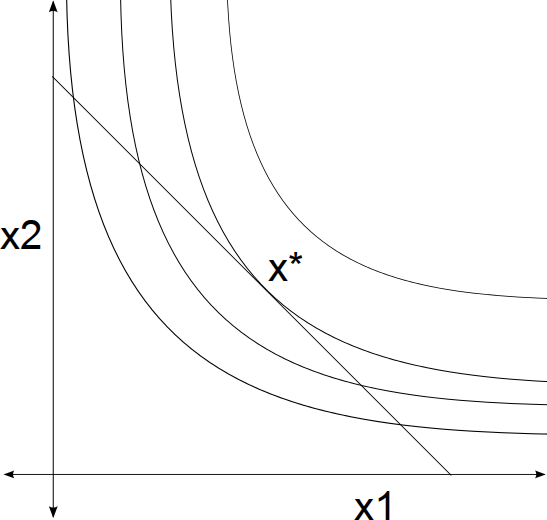
\includegraphics[width=0.5\textwidth]{indiff}
  \end{center}
\end{figure}

Now, let's look at a generic maximization problem with equality
constraints. \[ \max f(x) \text{ s.t. } h(x) = c \]
where $f: \R^n \to \R$ and $h: \R^n \to \R^m$. As in the unconstrained
case, consider a small perturbation of $x$ by some small $v$. The
function value is then approximately,
\[ f(x+v) \approx f(x) + Df_x v \]
and the constraint value is 
\[ h(x+v) \approx h(x) + Dh_x v \] $x+v$ will be satisfy the
constraint only if $Dh_xv = 0$. Thus, $x$ is a constrained local
maximum if for all $v$ such that $Dh_x v = 0$ we also have $Df_x v =
0$. 

Now, we want to express this condition in terms of Lagrange
multipliers. Remember that $Dh_x$ is an $m \times n$ matrix of partial
derivatives, and $Df_x$ is a $1 \times n$ row vector of partial
derivatives.  If $n=2$ and $m=1$ this condition can be written as
\[ \frac{\partial h}{\partial x_1} (x) v_1 + \frac{\partial
  h}{\partial x_2} (x) v_2 = 0 \]
implies
\[ \frac{\partial f}{\partial x_1} (x) v_1 + \frac{\partial
  f}{\partial x_2} (x) v_2 = 0. \]
Solving the first of these equations for $v_2$, substituting into the
second and rearranging gives
\[ \frac{ \frac{\partial f}{\partial x_1}(x) } { \frac{\partial
    h}{\partial x_1}(x) } = \frac{ \frac{\partial f}{\partial x_2}(x)}
{ \frac{\partial h}{\partial x_2}(x) }, \]
which as in the consumer example above, we can rewrite as
\begin{align*}
  \frac{\partial f}{\partial x_1} - \mu  \frac{\partial h}{\partial x_1} = & 0 \\
  \frac{\partial f}{\partial x_2} - \mu  \frac{\partial h}{\partial x_2} = & 0.
\end{align*}
for some constant $\mu$. Similar reasoning would show that for any $n$
and $m=1$, if for all $v$ such that $Dh_x v = 0$ we also have $Df_x v =
0$, then it is also true that there exists $\mu$ such that 
\[ \frac{\partial f}{\partial x_i} - \mu  \frac{\partial h}{\partial
  x_i} = 0 \] 
for  $i=1, ..., n$. Equivalently, using matrix notation $Df_x = \mu
Dh_x$. Note that conversely, if such a $\mu$ exists, then trivially
for any $v$ with $Dh_x v =0$, we have $Df_x v = \mu Dh_x v = 0$. 

When there are multiple constraints, i.e.\ $m>1$, it would be
reasonable to guess that $Dh_x v = 0$ implies $Df_x v = 0$ if and only
if there exists $\mu \in \R^m$ such that 
\begin{align*}
  \frac{\partial f}{\partial x_i} - \sum_{j=1}^m \mu_j  \frac{\partial
    h_j}{\partial x_i} = & 0 
\end{align*}
or in matrix notation $Df_x = \mu^T Dh_x$. This is indeed true. It is
tedious to show using algebra, but will be easy to show later using
some results from linear algebra about the row, column, and null
spaces of matrices. 

The following theorem formally states the preceding result.
\begin{theorem}[First order condition for maximization with equality
  constraints] \label{thm:econ} Let $f:\R^n \to \R$ and $h: \R^n \to
  \R^m$ be continuously differentiable. Suppose $x^*$ is a constrained
  local maximizer of $f$ subject to $h(x) = c$. Also assume that
  $Dh_{x^*}$ has rank $m$. Then there exists $\mu^* \in \R^m$ such
  that $(x^*, \mu^*)$ is a critical point of the Lagrangian,
  \[ L(x,\mu) = f(x) - \mu^T (h(x) - c). \]
  i.e.
  \begin{align*}
    \frac{\partial L}{\partial x_i}(x^*,\mu^*) = & \frac{\partial
      f}{\partial x_i} - {\mu^*}^T \frac{\partial h}{\partial
      x_i}(x^*) = 0 \\
    \frac{\partial L}{\partial \mu_j}(x^*,\mu^*) = & h(x^*) -
    c = 0
  \end{align*}
  for $i = 1, ..., n$ and $j=1,...,m$.
\end{theorem}
The assumption that $Dh_{x*}$ has rank $m$ is needed to make sure that
we don't divide by zero when defining the Lagrange multipliers. When
there is a single constraint, it simply says that at least one of the
partial derivatives of the constraint is non-zero. This assumption is
called the non-degenerate constraint qualification. It is rarely an
issue for equality constraints.

\begin{example}
  Solve the problem:
  \begin{align*}
    \max_{x} \alpha_1 \log x_1 + \alpha_2 \log x_2 \text{ s.t. } (p_1
    x_1 + p_2 x_2 - y)^3 = 0
  \end{align*}
\end{example}

\subsection{Lagrange multipliers as shadow prices}

Recall that in our example of consumer choice, the Lagrange multiplier
could be interpreted as the marginal utility of income.  A similar
interpretation will always apply. 

Consider a constrained maximization problem,
\[ \max_{x} f(x) \text{ s.t. } h(x) = c \]
From \ref{thm:econ}, the first order conditions are
\begin{align*}
 Df_{x^*} - \mu^T Dh_{x*} = & 0 \\
 h(x^*) - c = & 0.
\end{align*}
What happens to $x^*$ and $f(x^*)$ if $c$ changes? Let $x^*(c)$ denote
the maximizer as a function of $c$. Differentiating the constraint
with respect to $c$ shows that
\[ Dh_{x^*(c)} Dx^*_c = I \]
By the chain rule,
\[ D_c \left( f(x^*(c)) \right) = Df_{x^*(c)} Dx^*_c. \] 
Using the first order condition to substitute for $Df_{x^*(c)}$, we
have
\begin{align*}
  D_c \left( f(x^*(c)) \right) = & \mu^T Dh_{x^*(c)} Dx^*_c \\
  = & \mu^T 
\end{align*}
Thus, the multiplier, $\mu$, is the derivative of the maximized
function with respect to $c$.  In economic terms, the multiplier is
the marginal value of increasing the constraint. Because of this
$\mu_j$ is called the shadow price of $c_j$. 

\begin{example}[Cobb-Douglas utility \label{ex:cd-util}]
  Consider the consumer's problem in example \ref{ex:consumer} with
  Cobb-Douglas utility,
  \[ \max_{x_1,x_2} x_1^{\alpha_1} x_2^{\alpha_2} \text{ s.t. } p_1 x_1 + p_2
  x_2 = y \]
  The first order conditions are
  \begin{align*}
    \alpha_1 x_1^{\alpha_1 -1} x_2^{\alpha_2}- p_1 \mu & = 0 \\
    x_1^{\alpha_1} \alpha_2 x_2^{\alpha_2-1} - p_2 \mu & = 0  \\
    p_1 x_1 + p_2 x_2 - y & = 0
  \end{align*}
  Solving for $x_1$ and $x_2$ yields 
  \begin{align*}
    x_1 = & \frac{\alpha_1}{\alpha_1 + \alpha_2} \frac{y}{p_1} \\
    x_2 = & \frac{\alpha_2}{\alpha_1 + \alpha_2} \frac{y}{p_2}.
  \end{align*}
  The expenditure share of each good $\frac{p_j x_j}{y}$, is constant
  with respect to income. Many economists, going back to
  \cite{engel1857} have studied how expenditure shares vary with
  income. See \cite{lewbel2008} for a brief review and additional
  references. 

  If we solve for $\mu$, we find that 
  \begin{align*}
    \mu = & \frac{\alpha_1^{\alpha_1} \alpha_2^{\alpha_2}}
    {(\alpha_1 + \alpha_2)^{\alpha_1+\alpha_2}}
    \frac{y^{\alpha_1+\alpha_2 -1}} {p_1^{\alpha_1} p_2^{\alpha^2} }
  \end{align*}
  $\mu$ is the marginal utility of income in this model. As an
  exercise you may want to verify that if we were to take a monotonic
  transformation of the utility function (such as $\log(x_1^{\alpha_1}
  x_2^{\alpha_2})$ or $(x_1^{\alpha_1} x_2^{\alpha_2})^\beta$) and
  re-solve the model, then we would obtain the same demand functions,
  but a different marginal utility of income. 
\end{example}

\subsection{Inequality constraints}

Now let's consider an inequality instead of equality constraint. 
\[ \max_{x} f(x) \text{ s.t. } g(x) \leq b. \] 
When the constraints binds, i.e.\ $g(x^*) = b$, the situation is exactly the
same as with an equality constraint. However, the constraints do not
necessarily bind at a local maximum, so we must allow for that
possibility.  

Suppose $x^*$ is a constrained local maximum. To begin with, let's
consider a simplified case where there is only one constraint,
i.e. $g:\R^n \to \R$. If the constraint does not bind, then for small
changes to $x^*$, the constraint will still not bind. In other words,
locally it as though we have an unconstrained problem. Then, as in our
earlier analysis of unconstrained problems, it must be that $Df_{x^*}
= 0$. Now, suppose the constraint does bind. Consider a small change
in $x$, $v$. Since $x^*$ is a local maximum, it must be that if $f(x^*
+ v) > f(x^*)$, then $x^* + v$ must violate the constraint, $g(x^* +
v) > b$.  Taking first order expansions, we can say that if $Df_{x^*}
v > 0$, then $Dg_{x^*} v > 0$. This will be true if $Df_{x^*} =
\lambda Dg_{x^*}$ for some $\lambda > 0$. Note that the sign of the
multiplier $\lambda$ matters here. 

To summarize the results of the previous paragraph. If $x^*$ is a
constrained local maximum, then there exists $\lambda \geq 0$ such
that $Df_{x^*} - \lambda Dg_{x^*} = 0$. Furthermore if $\lambda > 0$, then
$g(x^*) = b$. If $g(x^*) < b$, then $\lambda = 0$ (it is also, but
rare possible for both $\lambda = 0$ and $g(x^*) = b$). This situation
where if one inequality is strict and then another holds with equality
and vice versa is called a complementary slackness condition. 

Essentially the same result holds with multiple inequality
constraints. 
 
\begin{theorem}[First order condition for maximization with inequality
  constraints] \label{thm:icon} 
  Let $f:\R^n \to \R$ and $g: \R^n \to \R^m$ be continuously
  differentiable. Suppose $x^*$ is a local maximizer of $f$ subject to 
  $g(x) \leq b$. Suppose that the first $k \leq m$ constraints, bind
  \[ g_j(x^*) = b_j \]
  for $j = 1 ... k$ and that the Jacobian for these constraints, 
  \[ \begin{pmatrix} 
    \frac{\partial g_1}{\partial x_1} &  \cdots &\frac{\partial g_1}{\partial x_n}  \\
    \vdots & & \vdots \\
    \frac{\partial g_k}{\partial x_1} &  \cdots &\frac{\partial g_k}{\partial x_n}  
  \end{pmatrix}
  \]
  has rank $k$. Then, there exists
  $\lambda^* \in \R^m$ such that for
  \[ L(x,\lambda) = f(x) - \lambda^T (g(x) - b). \]
  we have
  \begin{align*}
    \frac{\partial L}{\partial x_i}(x^*,\lambda^*) = & \frac{\partial
      f}{\partial x_i} - {\lambda^*}^T \frac{\partial g}{\partial
      x_i}(x^*) = 0 \\
    \lambda_j^* \frac{\partial L}{\partial \lambda_j}(x^*,\lambda^*) =
    & \lambda_j^* \left(g_j(x^*) - b \right)= 0 \\
    \lambda_j^* & \geq 0 \\
    g_j(x^*) & \leq b_j
  \end{align*}
  for $i = 1, ..., n$ and $j=1,...,m$. Moreover for each $j$ at least
  one of $\lambda_j^* \geq 0$ and $g_j(x^*) \leq b_j$ holds with
  equality (complementary slackness).
\end{theorem}
Some care needs to be taken regarding the sign of the multipliers and
the setup of the problem. Given the setup of our problem, $\max_x f(x)
\text{ s.t. } g(x) \leq b$, if we write the Lagrangian as
$L(x,\lambda) = f(x) - \lambda^T (g(x) - b)$, then the $\lambda_j \geq
0$. If we instead wrote the Lagrangian as $L(x,\lambda) = f(x) +
\lambda^T (g(x) - b)$, then we would get negative multipliers. If we
have a minimization problem, $\min_x f(x) \text{ s.t. } g(x) \leq b$,
the situation is reversed. $f(x) - \lambda^T(g(x) - b)$ leads to
negative multipliers, and $f(x) + \lambda^T(g(x) - b)$ leads to
positive multipliers. Reversing the direction of the inequality in the
constraint, i.e. $g(x) \geq b$ instead of $g(x) \leq b$, also switches
the sign of the multipliers.  Generally it is not very important if
you end up with multipliers with the ``wrong'' sign. You will still
end up with the same solution for $x$. The sign of the multiplier does
matter for whether it is the shadow price of $b$ or $-b$. 

To solve the first conditions of an inequality constrained
maximization problem, you would first guess which constraints do and
do not bind. Then you would impose $\lambda_j = 0$ for the non-binding
constraints and solve for $x$ and the remaining components
$\lambda$. If the resulting $x$ do lead to the constraints not binding
that you guessed not binding, then that $x$ is a possible local
maximum. To find all possible local maxima, you would have to repeat
this for all possible combinations of constraints binding or
not. There $2^m$ such possibilities, so this process can be
tedious. Fortunately, the economics of a problem often suggest which
constraints will bind, and you rarely actually need to investigate all
$2^m$ possibilities.

\begin{example}
  Let's solve
  \begin{align*}
    \max_x x_1 x_2 \text{ s.t. } & x_1^2 + 2x_2^2 \leq & 3 \\
    & 2 x_1^2 + x_2^2 \leq & 3
  \end{align*}
  The Lagrangian is
  \begin{align*}
    L(x,\lambda) = x_1x_2 - \lambda_1(x_1^2 + 2x_2^2 - 3) -
    \lambda_2(2 x_1^2 + x_2^2 - 3) 
  \end{align*}
  The first order conditions are
  \begin{align*}
    0 = & x_2 - 2\lambda_1 x_1 - 4\lambda_2 x_1 \\
    0 = & x_1 - 4\lambda_1 x_2 - 2\lambda_2 x_2  \\
    0 = & \lambda_1(x_1^2 + 2x_2^2 - 3) \\
    0 = & \lambda_2(2 x_1^2 + x_2^2 - 3) 
  \end{align*}
  Now, we must guess which constraints bind. Since the problem is
  symmetric in $x_1$ and $x_2$, it is reasonable to start by guessing that either
  both constraints or neither constraint will bind. If neither
  constraint binds, then $\lambda_1 = \lambda_2 = 0$, and the first
  order conditions imply $x_1 = x_2 = 0$. This results in a function
  value of $0$. This is feasible, but it is not the maximum since for
  example, small positive $x_1$ and $x_2$ would also be feasible and
  give a higher function value. 

  Instead, suppose both constraints bind. Then the solutions to 
  $x_1^2 + 2x_2^2 = 3$ and $2 x_1^2 + x_2^2 = 3$ are $x_1 = \pm 1$ and
  $x_2 = \pm 1$. Substituting into the first order condition and
  solving for $\lambda_1$ and $\lambda_2$ gives
  \begin{align*} 
    0 = & 1 - 2 \lambda_1 - 4\lambda_2 \\
    0 = & 1 - 4 \lambda_1 - 2\lambda_2 \\
    \frac{1}{6} = & \lambda_1 = \lambda_2
  \end{align*}
  Both $\lambda_1$ and $\lambda_2$ are positive, so complementary
  slackness is satisfied.

  Finally, let's consider the case where the first constraint binds
  but not the second. In this case $\lambda_2 = 0$, and taking the
  ratio of the first order conditions gives
  \begin{align*} 
    \frac{x_2}{x_1} = & \frac{1}{2} \frac{x_1}{x_2}
  \end{align*}
  or $x_2^2 = \frac{1}{2} x_1^2$. Substituting this into the first
  constraint yields $x_1^2 + x_1^2 = 3$ , so $x_1 = \sqrt{3/2}$, and
  $x_2 = \sqrt{3/4}$. However, then $2x_1^2 + x_1^2 = 3 + 3/4 >
  3$. The second constraint is violated, so this cannot be the solution.   
\end{example}

\begin{example}
  Show that replacing the problem 
  \[ \max_x f(x) \text{ s..t } g(x) \leq b. \]
  with an equality constrained problem with slack variables $s$, 
  \[ \max_{x,s} f(x) \text{ s..t } g(x) - s = b, \]
  leads to the same conclusions are theorem \ref{thm:icon}
\end{example}


\subsection{Second order conditions}


\section{Envelope theorem}


\appendix

\section{Notation \label{sec:notation}}
\begin{itemize}
\item $\R$ is the set of real numbers $\R^n$ is the set of
  vectors of $n$ real numbers.
\item $x \in \R^k$ is read ``x in $\R^k$'' and means that $x$ is
  vector of $k$ real numbers.
\item $f: \R^n \to \R$ means $f$ is a function from $\R^n$ to
  $\R$. That is, $f$'s argument is an n-tuple of real numbers and
  its output is a single real number.
\item When convenient we will treat $x \in \R^k$ as a $k \times 1$
  matrix, so $w^T x = \sum_{i=1}^k w_i x_i$
\end{itemize}


\section{Review of derivatives \label{sec:derivatives}}
Partial and directional derivatives were discussed on the summer math
review, so we will just briefly restate their definitions and some key
facts here.
\begin{definition}
  Let $f:\R^n \to R$. The $i$th \textbf{partial derivative} of $f$
  is
  \[ \frac{\partial f}{\partial x_i} (x_0) = \lim_{h \to 0}
  \frac{f(x_{01},...,x_{0i}+h, ... x_{0n}) - f(x_0) }{h}. \]
\end{definition}
The $i$th partial derivative tells you how much the function changes
as its $i$th argument changes. 
\begin{definition}
  Let $f: \R^n \to \R^k$, and let $v \in \R^n$ the \textbf{directional
    derivative} in direction $v$ at $x$ is
  \begin{align*}
    df(x;v) = \lim_{\alpha \to 0} \frac{f(x + \alpha v) - f(x)}{\alpha}.
  \end{align*}  
  where $\alpha \in \R$ is a scalar.
\end{definition}
An important result relating partial to directional derivatives is the
following.
\begin{theorem}\label{thm:pddiff}
  Let $f:\R^n \to \R$ and suppose its partial derivatives exist and
  are continuous in a neighborhood of $x_0$. Then
  \[ df(x;v) = \sum_{i=1^n} v_i \frac{\partial f}{\partial x_i}
  (x_0) \]
  in this case we will say that $f$ is differentiable at $x_0$.
\end{theorem}

It is convenient to gather partial derivatives of a function into a
matrix. For a function $f: R^n \to \R$, we will gather its partial
derivatives into a $1 \times n$ matrix, 
\[ Df_x = \begin{pmatrix} \frac{\partial f}{\partial x_1}(x) & \cdots
  & \frac{\partial f}{\partial x_n}(x)
\end{pmatrix}. \]
We will simply call this matrix the derivative of $f$ at $x$. This
helps reduce notation because for example we can write
\[ df(x;v) = \sum_{i=1^n} v_i \frac{\partial f}{\partial x_i}
(x_0) = Df_x v. \]

Similarly, we can define second and higher order partial and
directional derivatives.
\begin{definition}
  Let $f:\R^n \to R$. The $ij$th \textbf{partial second derivative} of $f$
  is 
  \[ \frac{\partial^2 f}{\partial x_i \partial x_j} (x_0) = \lim_{h \to 0}
  \frac{\frac{\partial f}{\partial x_i} (x_{01},...,x_{0j}+h, ... x_{0n}) -
    \frac{\partial f}{\partial x_i}(x_0) }{h}. \] 
\end{definition}
\begin{definition}
  Let $f: \R^n \to \R^k$, and let $v, w \in \R^n$ the \textbf{directional
    derivative} in directions $v$ and $w$ at $x$ is
  \begin{align*}
    d^2f(x;v,w) = \lim_{\alpha \to 0} \frac{df(x + \alpha w;v) - df(x;v)}{\alpha}.
  \end{align*}  
  where $\alpha \in \R$ is a scalar.
\end{definition}
\begin{theorem}\label{thm:pddiff2}
  Let $f:\R^n \to \R$ and suppose its first and second partial
  derivatives exist and are continuous in a neighborhood of
  $x_0$. Then
  \[ d^2f(x;v,w) = \sum_{j=1}^n \sum_{i=1^n} v_i \frac{\partial^2
    f}{\partial x_i \partial x_j}
  (x_0) w_j \]
  in this case we will say that $f$ is twice differentiable at $x_0$. 
  Additionally, if $f$ is twice differentiable, then $\frac{\partial^2
    f}{\partial x_i \partial x_j} = \frac{\partial^2
    f}{\partial x_j \partial x_j}$.
\end{theorem}
We can gather the second partials of $f$ into an $n \times n$ matrix,
\[ D^2 f_{x} = \begin{pmatrix} \frac{\partial ^2 f}{\partial x_1^2}
  & \cdots & \frac{\partial^2 f }{\partial x_1\partial x_n} \\
  \vdots & \ddots & \vdots \\
  \frac{\partial^2 f}{\partial x_1\partial x_n} & \cdots &
  \frac{\partial^2 f}{\partial x_n}^2 \end{pmatrix},
\]
and then write $d^2f(x;v,w) = w^T D^2 f_x w$. $D^2 f_x$ is also called
the Hessian of $f$.

\clearpage
\bibliographystyle{jpe}
\bibliography{../526}

\end{document}
